\documentclass{article}
\usepackage{tikz}
\usetikzlibrary{arrows.meta}

\begin{document}

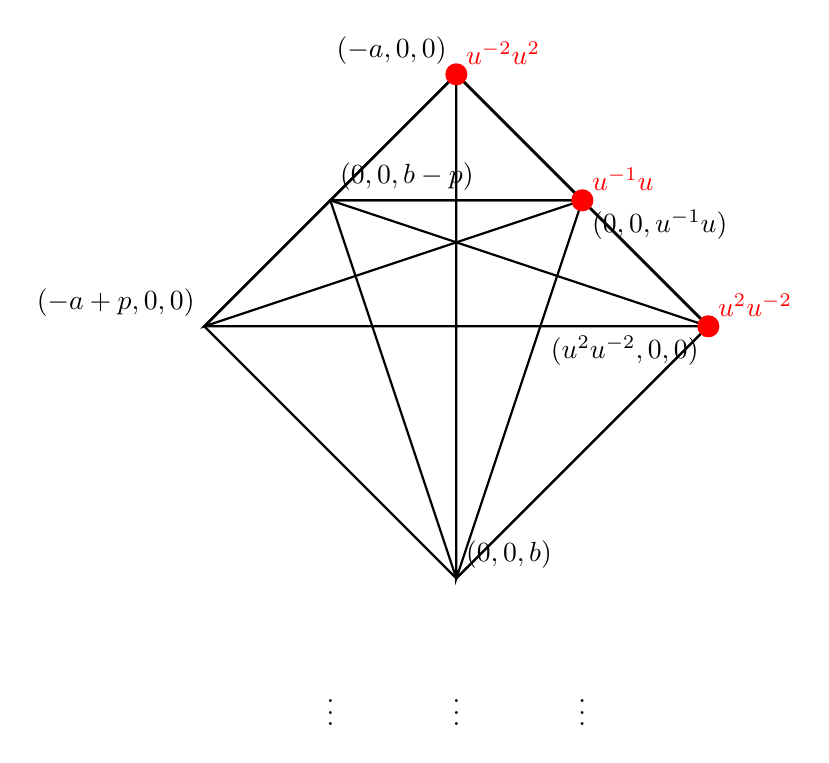
\begin{tikzpicture}[scale=0.8]
    % Define coordinates for the vertices
    \coordinate (A) at (0,0);
    \coordinate (B) at (-4,4);
    \coordinate (C) at (-2,6);
    \coordinate (D) at (0,8);
    \coordinate (E) at (2,6);
    \coordinate (F) at (4,4);
    
    % Draw the lattice structure
    \draw[thick] (A) -- (B) -- (C) -- (D) -- (E) -- (F) -- cycle;
    \draw[thick] (A) -- (C) -- (E) -- (F) -- cycle;
    \draw[thick] (B) -- (D) -- (F) -- cycle;
    \draw[thick] (A) -- (D) -- (E) -- cycle;
    \draw[thick] (B) -- (C) -- (E) -- cycle;
    \draw[thick] (C) -- (D) -- (F) -- cycle;
    
    % Label the vertices
    \node at (A) [above right] {$(0,0,b)$};
    \node at (B) [above left] {$(-a+p,0,0)$};
    \node at (C) [above right] {$(0,0,b-p)$};
    \node at (D) [above left] {$(-a,0,0)$};
    \node at (E) [below right] {$(0,0,u^{-1}u)$};
    \node at (F) [below left] {$(u^2u^{-2},0,0)$};
    
    % Draw the red dots with labels
    \fill[red] (E) circle (5pt) node[above right] {$u^{-1}u$};
    \fill[red] (F) circle (5pt) node[above right] {$u^2u^{-2}$};
    \fill[red] (D) circle (5pt) node[above right] {$u^{-2}u^2$};
    
    % Add the ellipsis
    \node at (0,-2) {$\vdots$};
    \node at (2,-2) {$\vdots$};
    \node at (-2,-2) {$\vdots$};
\end{tikzpicture}

\end{document}